%!TEX root = ../thesis.tex

\chapter{Annexes}

\graphicspath{{Appendix1/Appendix1Figs/PNG/}{Appendix1/Appendix1Figs/PDF/}{Appendix1/Appendix1Figs/}}

\begin{figure}[ht]
  \begin{center}
    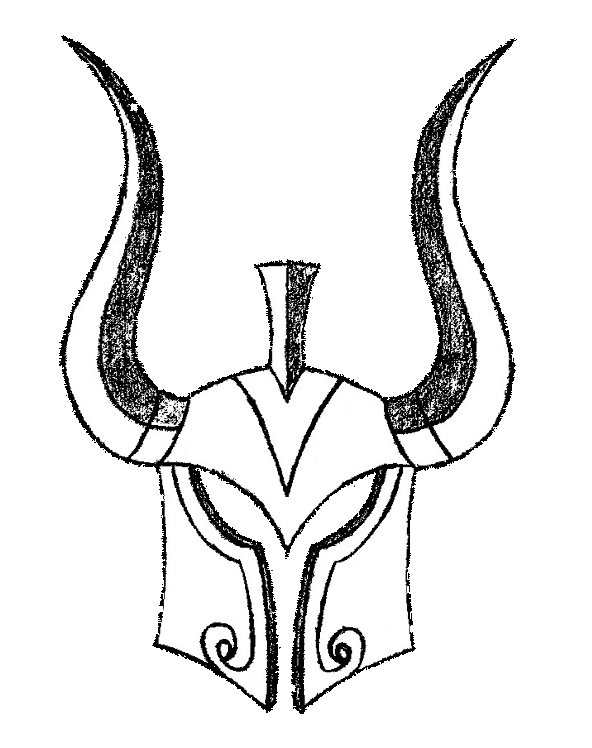
\includegraphics[scale=0.2]{Deformation-Capricorne-Avant}
    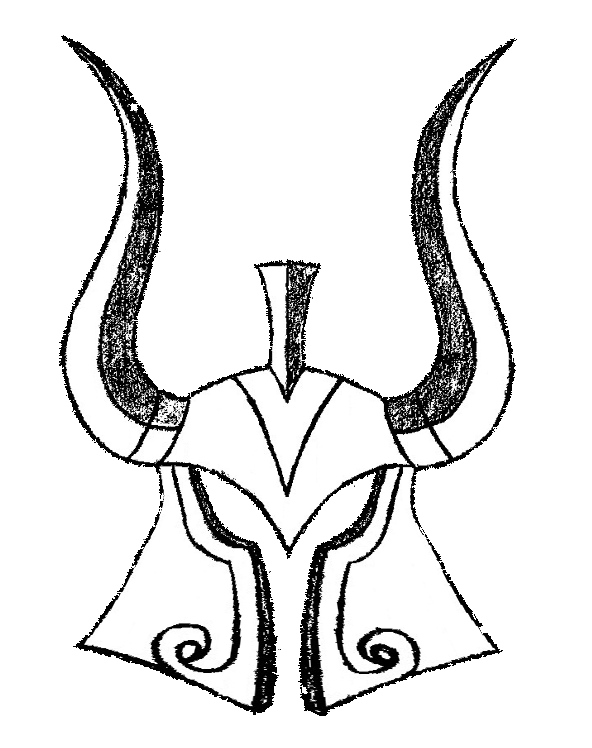
\includegraphics[scale=0.2]{Deformation-Capricorne-Apres}

    \caption{Exemple de déformation avec une cage de contrôle d'influence. A
gauche le casque avant déformation, à droite après déformation de la
partie basse du casque.}

  \end{center}
\end{figure}

\begin{figure}[ht]
  \begin{center}
    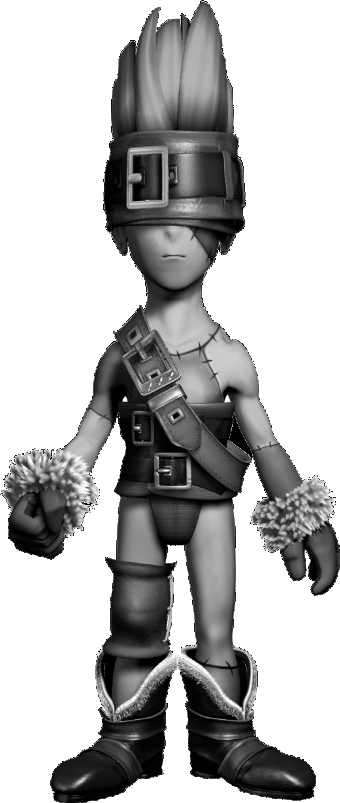
\includegraphics[scale=0.3]{Deformation-Frank-Tete}
    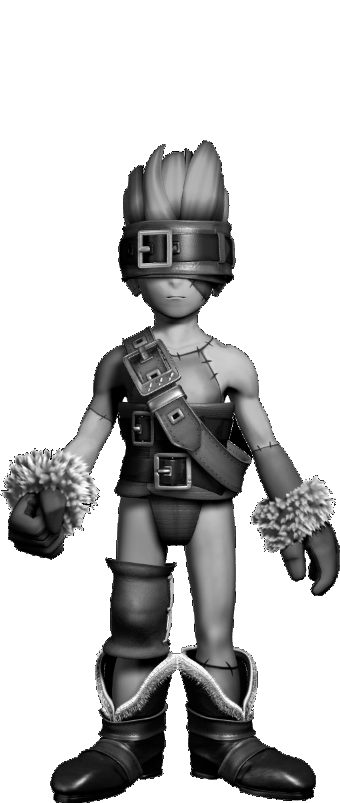
\includegraphics[scale=0.3]{Deformation-Frank-Avant}
    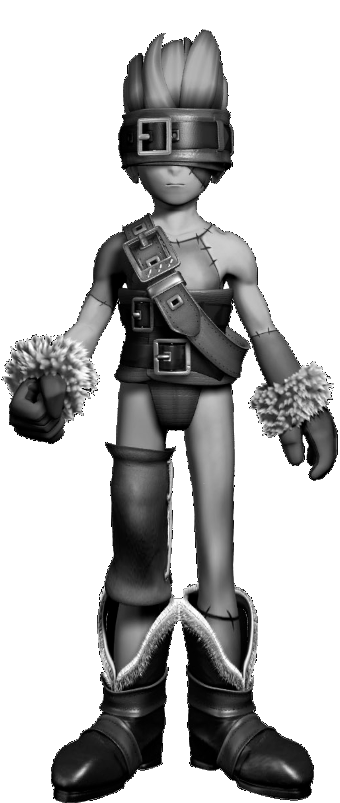
\includegraphics[scale=0.3]{Deformation-Frank-Jambes}

    \caption{Exemple de déformation avec deux cages de contrôle d'influence.
Au milieu le personnage avant déformation, à gauche après déformation de
la tête, à droite après déformation des jambes.}

  \end{center}
\end{figure}

% ------------------------------------------------------------------------